% Figure -- T-D trade-off envelope (designable vs whole-set pwTM). Optional/appendix;
% superseded in the main text by tables/table_concentration.tex. \input{} where used.
\begin{figure}[tbp]
\centering
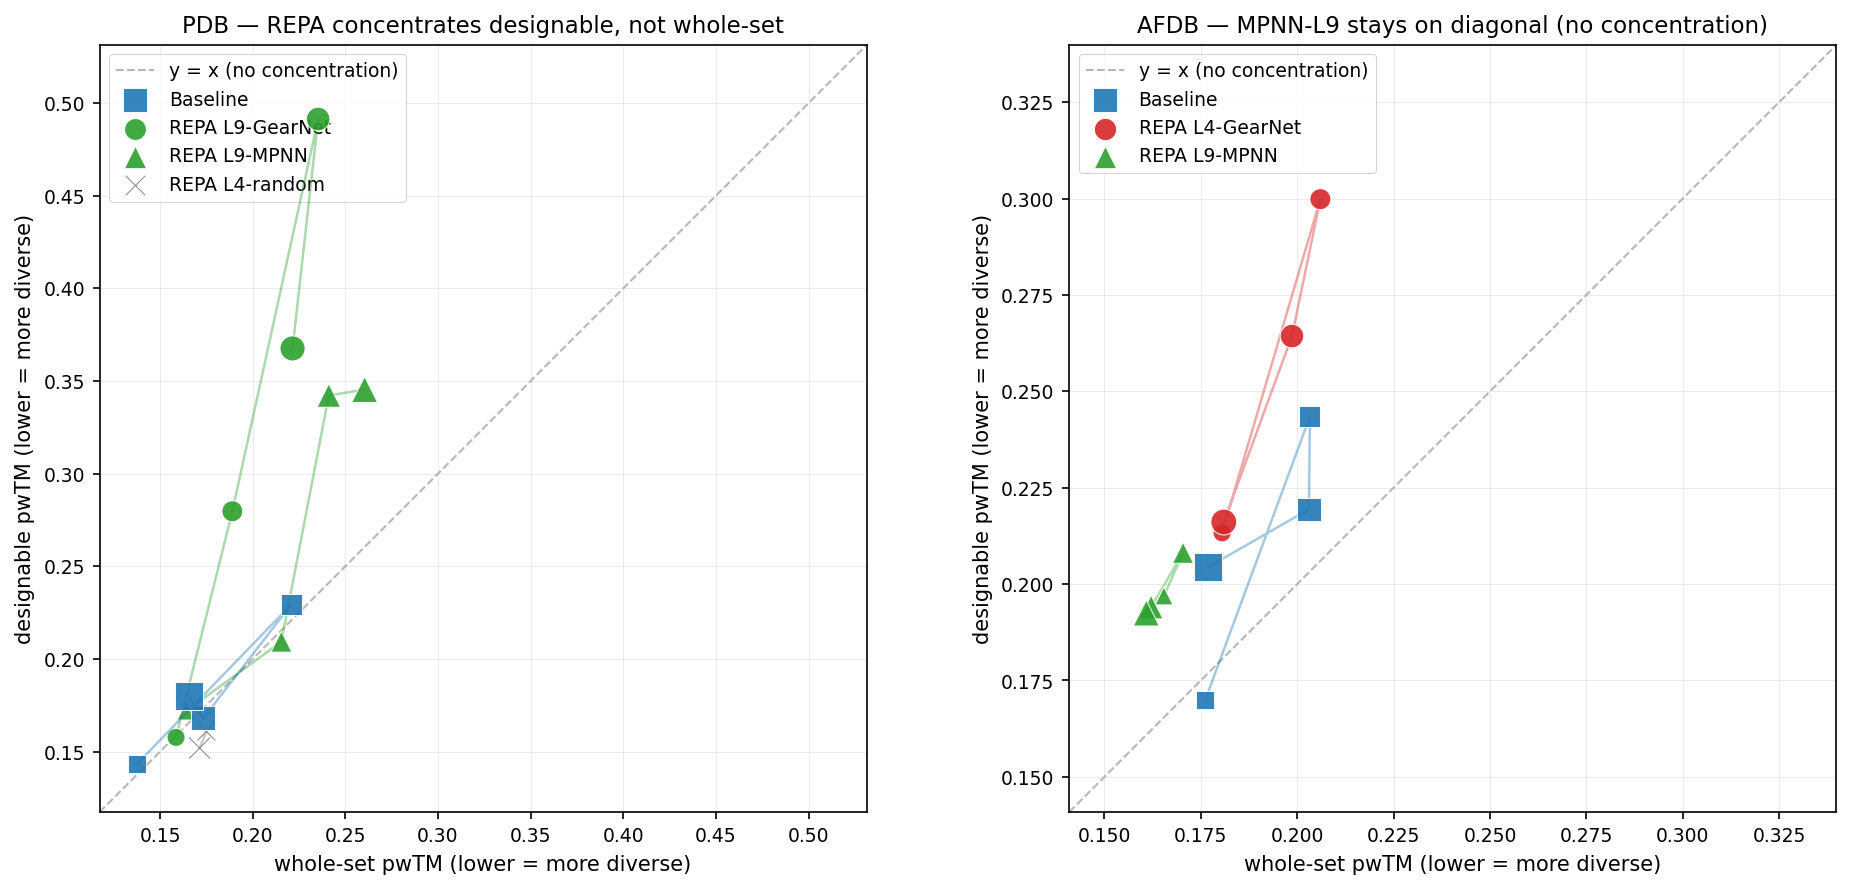
\includegraphics[width=\textwidth]{figures/fig05_td_tradeoff.png}
\caption{\textbf{REPA concentrates the designable subset onto fewer folds --- points rise above the diagonal --- except the AFDB-MPNN falsifier, which stays on it.} Designable-subset pairwise TM-score against whole-set pairwise TM-score (both lower = more diverse), one marker per checkpoint; points above the $y=x$ diagonal mean the designable subset is less diverse than the whole set. \emph{Left:} on PDB, REPA (GearNet circles, MPNN triangles) departs well above the diagonal while the baseline sits on it. \emph{Right:} on AFDB, MPNN-L9 stays on the diagonal --- the clean falsifier that escapes the trade-off --- while GearNet concentrates.}
\label{fig:proteina-tradeoff}
\end{figure}
